\documentclass[12pt]{beamer} %Makes presentation
%\documentclass[handout]{beamer} %Makes Handouts
%\setbeameroption{notes on second screen} %Dual-Screen Notes
%\setbeameroption{show only notes} %Notes Output

% white on black
\setbeamercolor{normal text}{fg=white,bg=blue!20!black}
\setbeamercolor{structure}{fg=white}
\setbeamercolor{alerted text}{fg=red!85!black}
%\setbeamercolor{item projected}{use=item,fg=black,bg=item.fg!35}
\setbeamercolor*{palette primary}{use=structure,fg=structure.fg}
\setbeamercolor*{palette secondary}{use=structure,fg=structure.fg!95!black}
\setbeamercolor*{palette tertiary}{use=structure,fg=structure.fg!90!black}
\setbeamercolor*{palette quaternary}{use=structure,fg=structure.fg!95!black,bg=black!80}
\setbeamercolor*{framesubtitle}{fg=white}
\setbeamercolor*{block title}{parent=structure,bg=black!60}
\setbeamercolor*{block body}{fg=black,bg=black}
\setbeamercolor*{block title alerted}{parent=alerted text,bg=black!15}
\setbeamercolor*{block title example}{parent=example text,bg=black!15}

% black on white
%\usetheme{Singapore} %Gray with fade at top
%\usecolortheme{seagull} %Color theme
%\usecolortheme{rose} %Inner color theme
\setbeamercolor{item}{fg=black!65}
%\setbeamercolor{enumerate item}{fg=black!55}

\useoutertheme[subsection=false]{miniframes} %Supppress subsection in header
\useinnertheme{rectangles} %Itemize/Enumerate boxes
\setbeamertemplate{navigation symbols}{}
\setbeamertemplate{mini frames}[default]
\setbeamercovered{dynamics}
\setbeamerfont*{title}{size=\Large,series=\bfseries}
%\setbeamertemplate{headline}{}

\newcommand{\heading}[1]{\noindent \textbf{#1}\\ \vspace{1em}}

\usepackage{bbding,color,multirow,times,ccaption,tabularx,graphicx,verbatim} %graphics,
\usepackage{colortbl}%Table overlays
\usepackage[english]{babel}

% font
\usepackage{tgadventor}
\renewcommand*\familydefault{\sfdefault} %% Only if the base font of the document is to be sans serif
\usepackage[T1]{fontenc}


\title[]{Introduction to R}

\begin{document}

\begin{frame}
	\titlepage
\end{frame}

\frame{}
\frame{\tableofcontents}

\section{Challenges}
\frame{\tableofcontents[currentsection]}

\frame{
\frametitle{Frustrations with your current software}
\begin{itemize}\itemsep2em
\item What frustrations {\bf did} you have learning your current software?
\item What frustrations {\bf do you still have} with your current software?
\end{itemize}
}


\frame{
\frametitle{Frustrations you will have with R}
\begin{itemize}\itemsep1em
\item<1-> No graphical user interface (GUI)
\item<2-> Lots of add-on packages (lightweight base software)
\item<3-> Mistype or misspell commands
\item<4-> Missing data handling
\item<5-> Cryptic error messages
\end{itemize}
}


\section{Opportunities}
\frame{\tableofcontents[currentsection]}

\frame<1>[label=whyr]{
\frametitle{Why should you use R?}
\begin{itemize}\itemsep2em
\item<1-> Because you want to do more
\item<2-> Because you can create a better scientific workflow
\item<3-> Because everyone else is doing it
\item<4-> Because it is free
\item<5-> Because R is beautiful
\end{itemize}
}


\frame{
\frametitle{What can you do with R?}
\begin{itemize}\itemsep2em
\item<2-> Everything
\end{itemize}
\vspace{1em}
\only<3->{But seriously\dots}
\vspace{1em}
\begin{itemize}
\item<4-> Everything\only<5->{:}
\vspace{1em}
	\begin{itemize}
	\item<5-> Statistical analysis
	\item<6-> Texting processing
	\item<7-> Machine learning
	\item<8-> Online data
	\item<9-> High-level visualization
	\item<10-> Sudoku
	\end{itemize}
\end{itemize}
}

\againframe<1-2>{whyr}

\frame{
\frametitle{Why is R better for science?}
\begin{itemize}\itemsep2em
\item R will always be here
\item Scripting
\item Reproducible research tools
	\begin{itemize}
	\item Scripting
	\item Report generation
	\item Data sharing
	\end{itemize}
\end{itemize}
}

\frame{
\frametitle{Reproducible Research}
\begin{itemize}\itemsep2em
\item All data and replication code is public
\item All results come directly from code
\item Analysis is about writing a script, not pointing and clicking
\item Makes changes and collaboration easier
\end{itemize}
}

\frame{
\frametitle{Scientific Workflow}
\begin{itemize}\itemsep2em
\item Store data in perpetually readable formats
\item Write a complete analysis script
\item Script should run analysis \emph{and} output results
\item Reports should import results directly
\item Share data, script, and codebooks
\end{itemize}
}

\frame[label=q]{\Large Questions so far?}

\againframe<2-3>{whyr}


\frame{
\frametitle{What is everyone else doing?}
\begin{center}
\only<1>{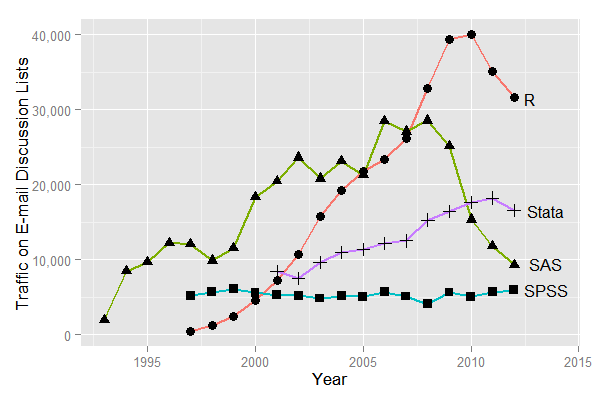
\includegraphics[width=\textwidth]{figure/rpop_listserv.png}}
\only<2>{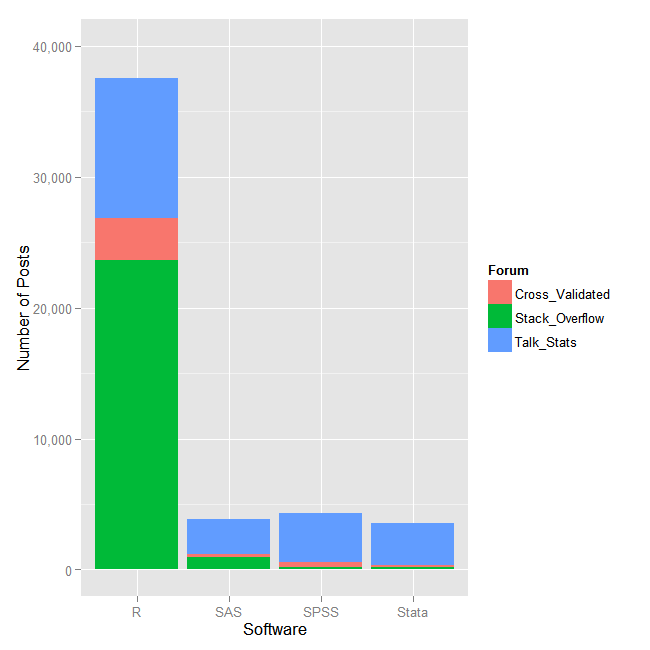
\includegraphics[height=.85\textheight]{figure/rpop_forum.png}}
%\only<3>{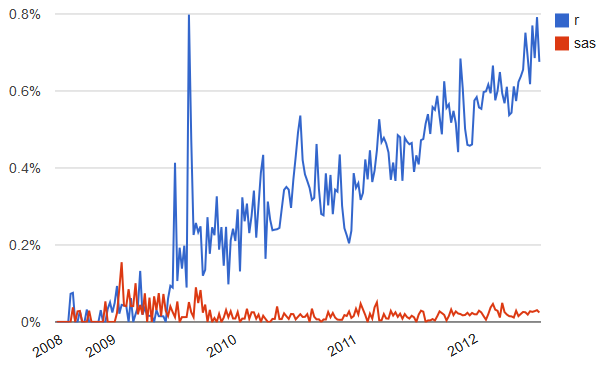
\includegraphics[width=\textwidth]{figure/rpop_so.png}}
%\only<4>{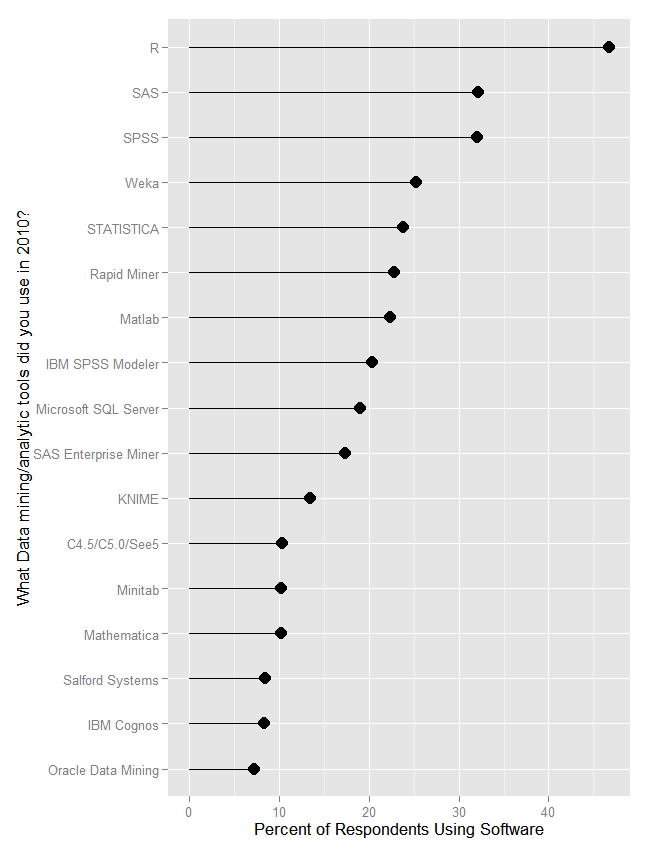
\includegraphics[height=.85\textheight]{figure/rpop_survey.png}}
%\only<5>{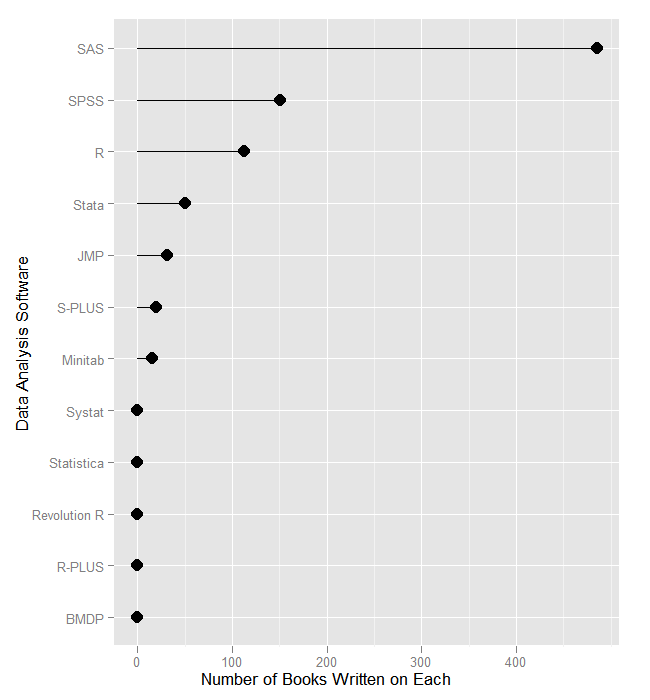
\includegraphics[height=.85\textheight]{figure/rpop_books.png}}
\only<6>{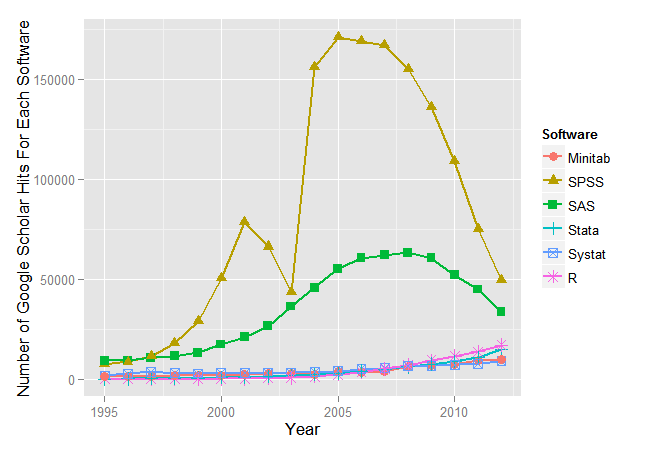
\includegraphics[width=\textwidth]{figure/rpop_gs.png}}
\only<7>{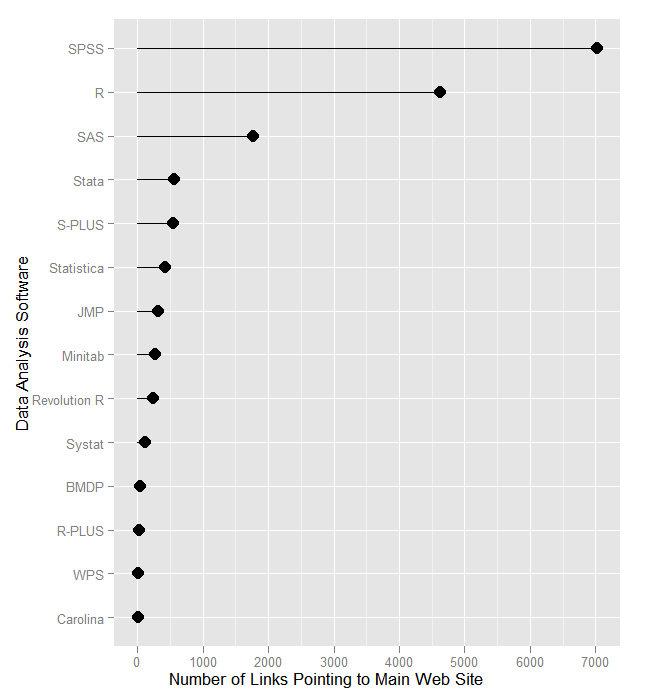
\includegraphics[height=.85\textheight]{figure/rpop_links.png}}
\end{center}
}

\frame{
\frametitle{Impact of popularity}
\begin{itemize}\itemsep2em
\item Huge community support
\item Cutting edge techniques
\item Versatile
\end{itemize}
}


\againframe<3-4>{whyr}

\frame{
\frametitle{What is freedom?}
\begin{itemize}\itemsep2em
\item<1-> Freedom means free
\item<2-> Freedom means forever
\item<3-> Freedom means independence
\item<4-> Freedom means control
\end{itemize}
}

\againframe<4-5>{whyr}

\frame{
\frametitle{Graphs are beautiful}
You can make data look like art
}


\bgroup
\setbeamercolor{background canvas}{bg=white}
\setbeamertemplate{navigation symbols}{}
\frame{
\begin{center}
%\only<1>{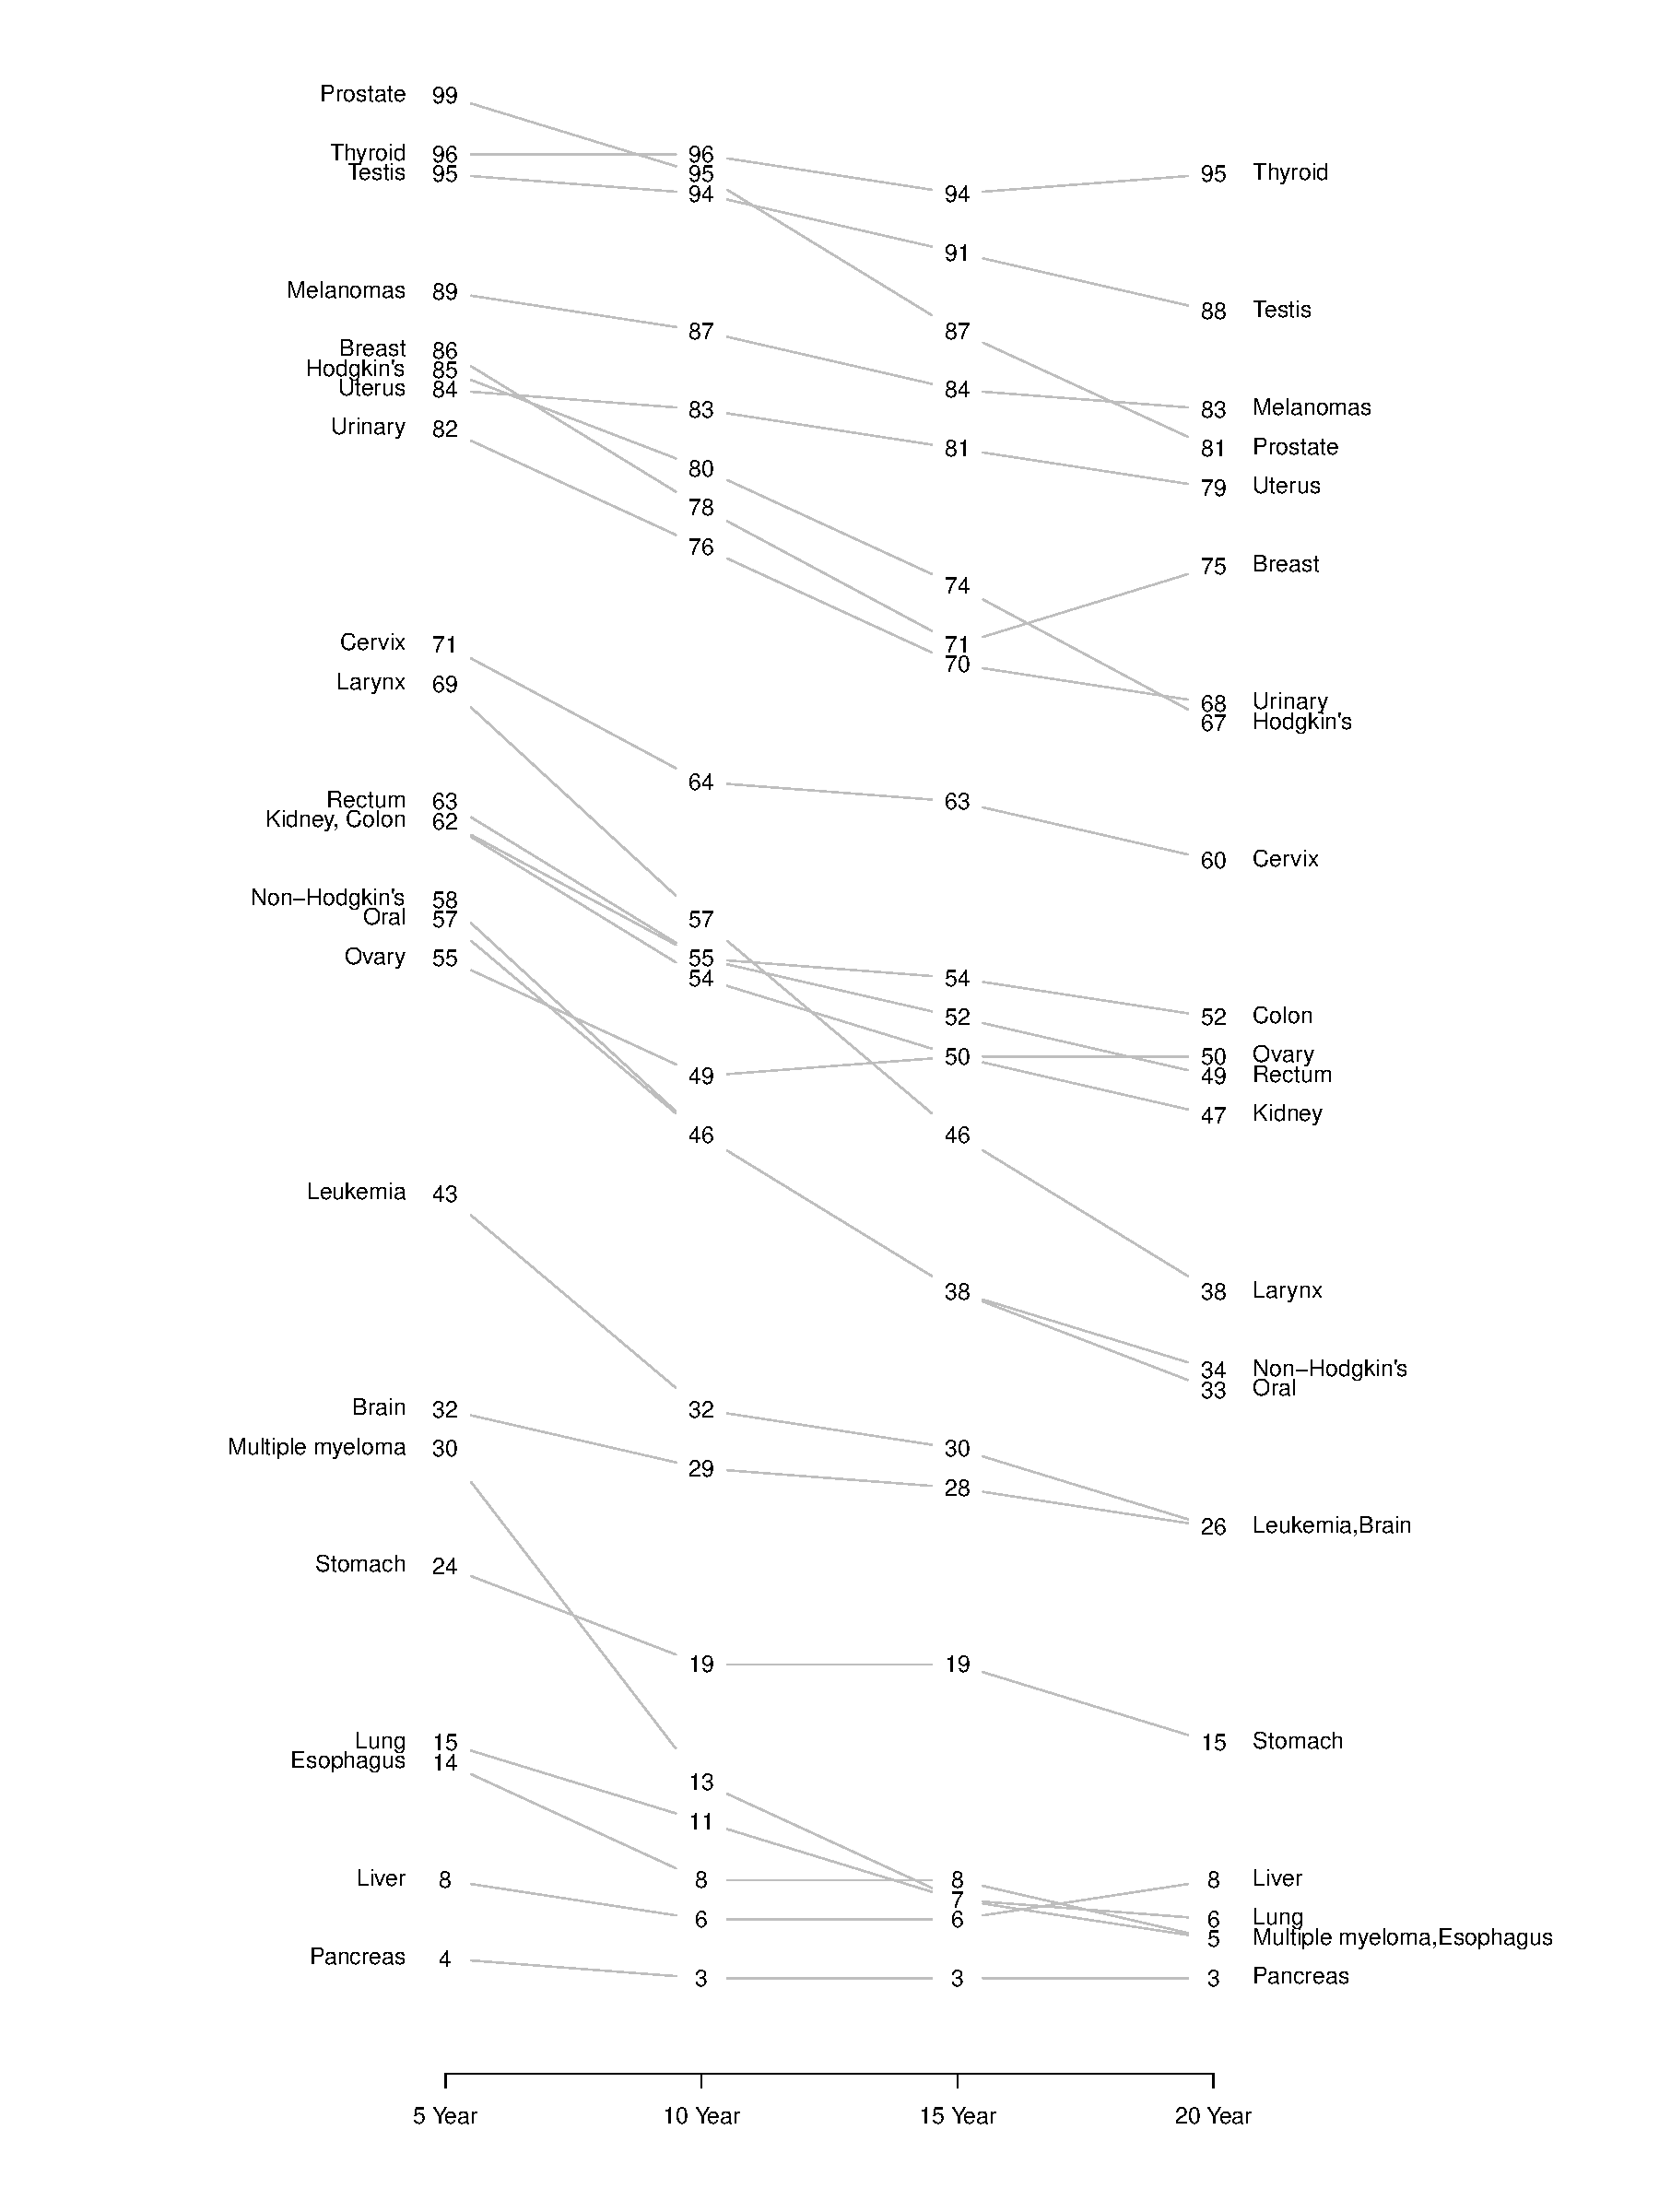
\includegraphics[height=\textheight]{figure/tufte-cancer-survival-plot.pdf}}
\only<1>{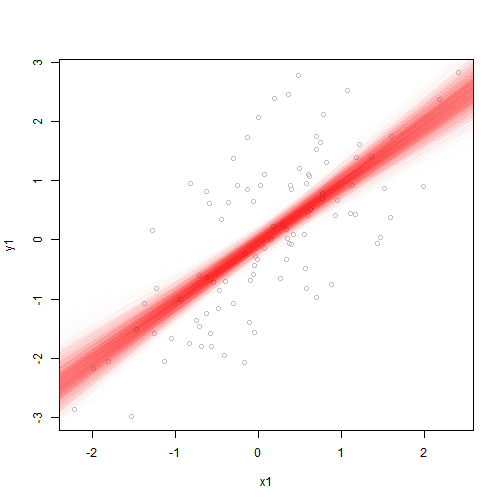
\includegraphics[height=\textheight]{figure/bootstrap_lm_fits.png}}
\only<2>{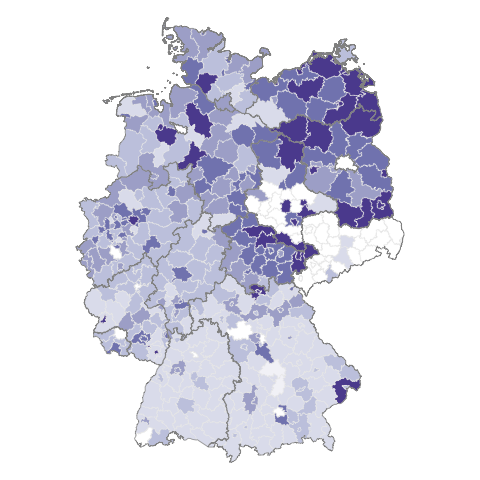
\includegraphics[height=\textheight]{figure/german_unemployment.png}}
\only<3>{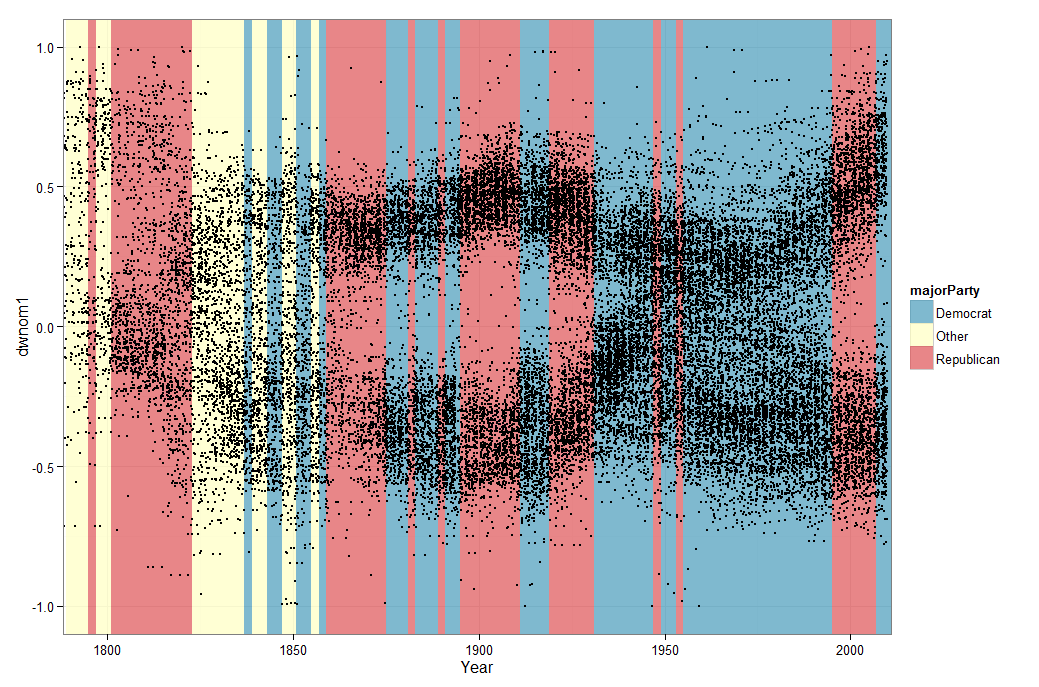
\includegraphics[width=\textwidth]{figure/nominate.png}}
\only<4>{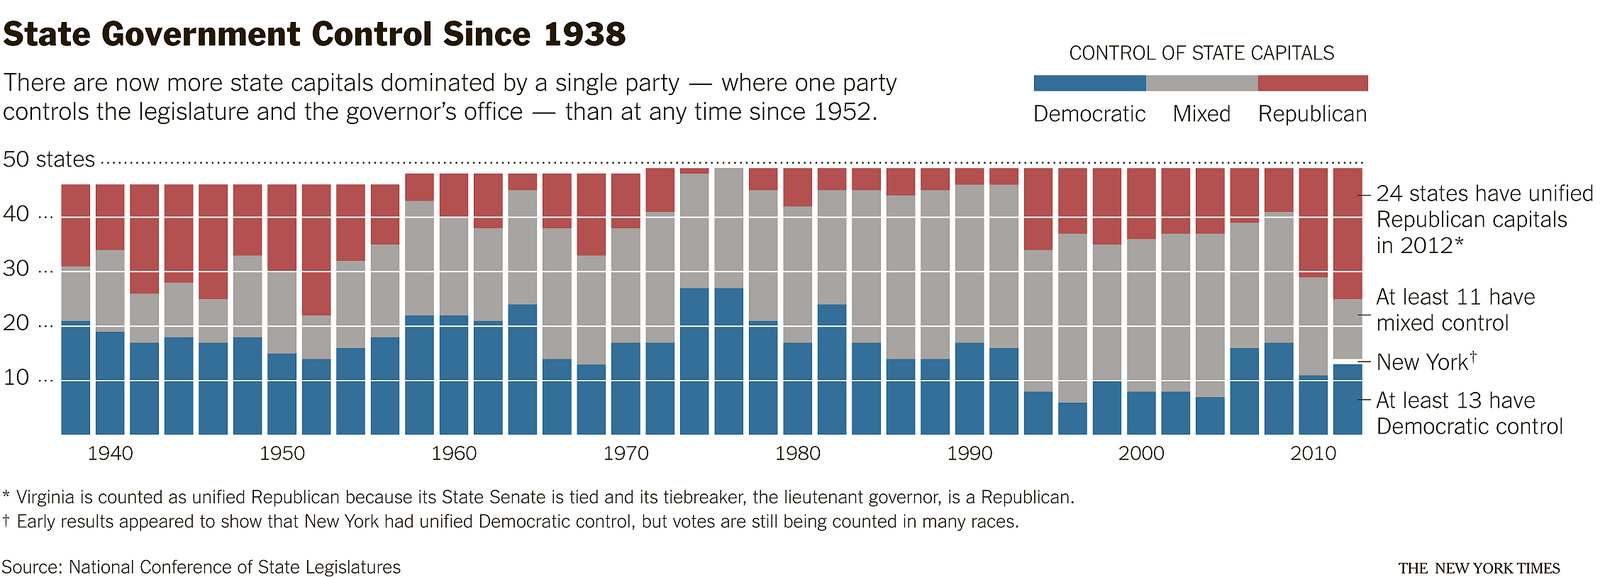
\includegraphics[width=\textwidth]{figure/nyt_govt_control.png}}
\only<5>{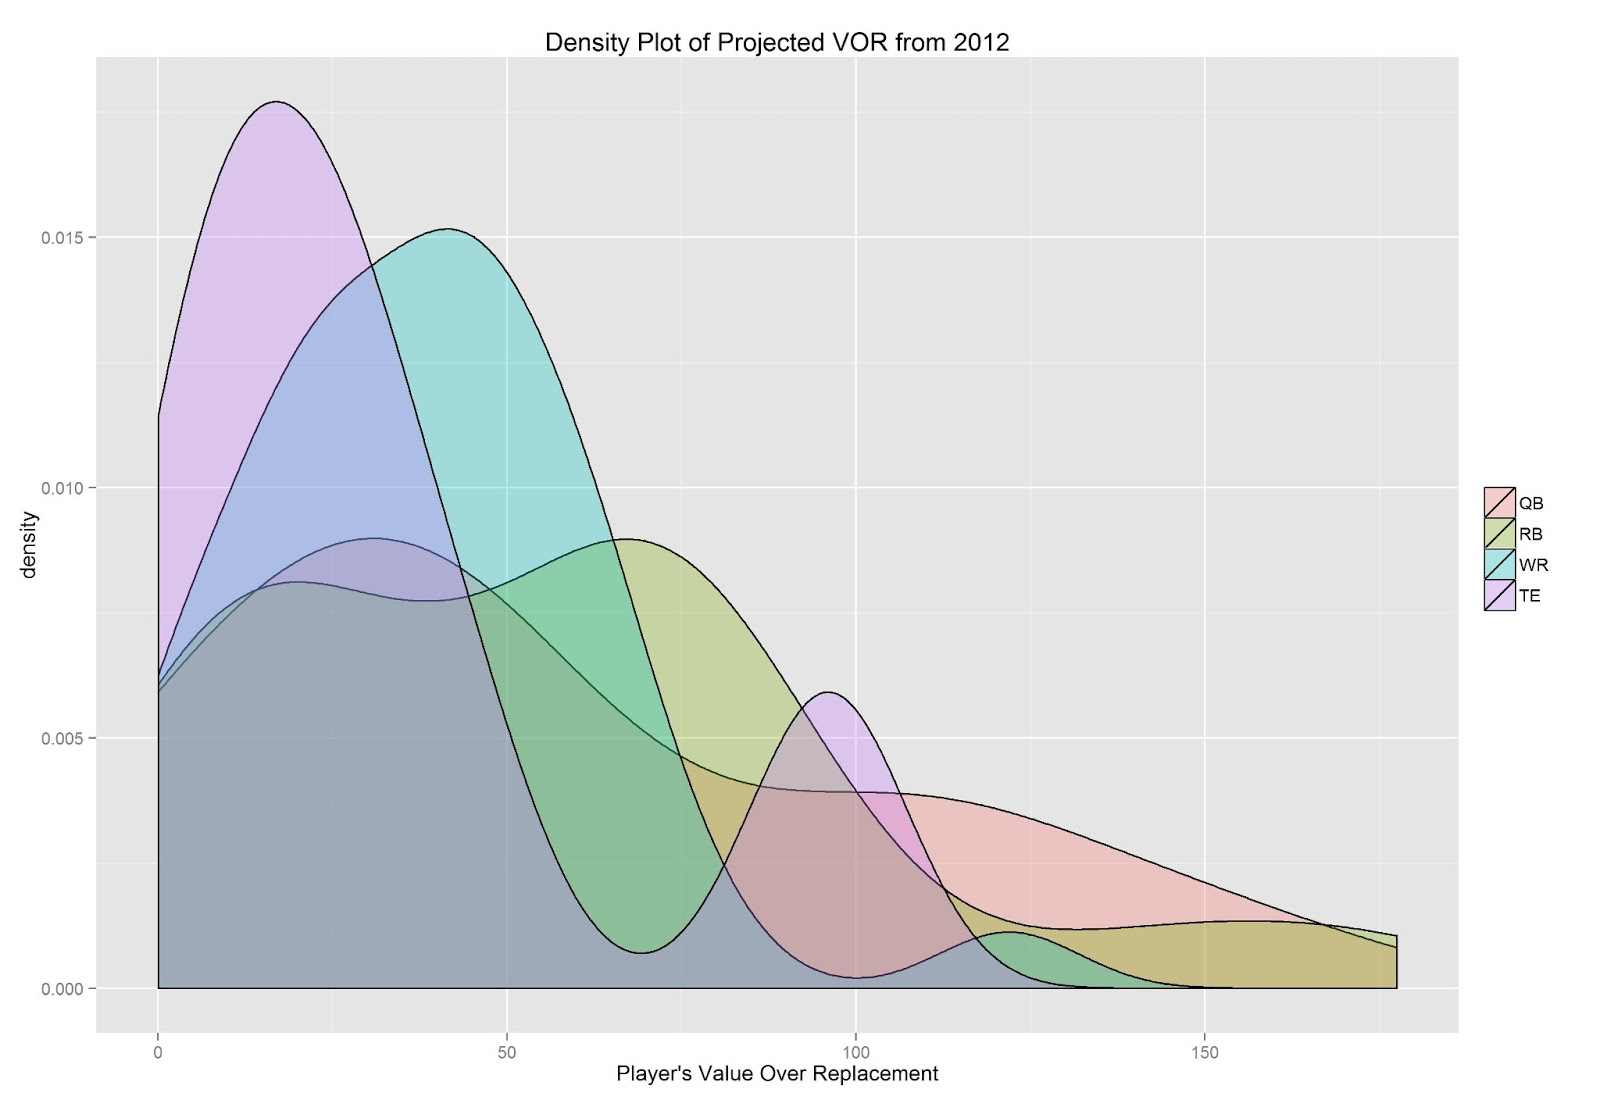
\includegraphics[width=\textwidth]{figure/playervalue.png}}
\end{center}
}
\egroup

\begin{comment}
\frame{
\frametitle{Code is beautiful}
\small
\begin{quote}
install.packages("knitr", repos="http://cran.r-project.org")\\
library(knitr)\\
setwd(tempdir())\\
s <- spin(text="\\
summary(lm(mpg \textasciitilde hp,data=mtcars))\\
with(mtcars, plot(mpg \textasciitilde hp))\\
out <- replicate(1000, with(mtcars[sample(1:nrow(mtcars),nrow(mtcars),TRUE),], abline(lm(mpg \textasciitilde hp),col=rgb(1,0,0,.1))))\\
", format="Rmd")\\
cat(s, file=t <- tempfile(fileext = ".html"))\\
browseURL(t)
\end{quote}
}
\end{comment}

\againframe{q}


%\appendix

\bgroup
\setbeamercolor{background canvas}{bg=black}
\setbeamertemplate{navigation symbols}{}
\begin{frame}[plain]{}
\end{frame}
\egroup

\end{document}
